\chapter{Methodology}

\section{Problem Formulation}

We formally define the problem of determining the partial ordering of code edits within a set, denoted as \(\mathbf{H}\). Given two elements \( h_i, h_j \in \mathbf{H} \), we aim to establish the relationship between these edits in terms of their sequence or independence. This relationship is defined by a function \( f(h_i, h_j) \) that categorizes the interactions between pairs of edits as follows:
\[
f(h_i, h_j) =
\begin{cases}
    h_i \rightarrow h_j, & \text{if } h_i \text{ must occur before } h_j \\
    h_i \leftarrow h_j, & \text{if } h_j \text{ must occur before } h_i \\
    h_i \leftrightarrow h_j, & \text{if either } h_i \text{ or } h_j \text{ can occur first (no strict order)} \\
    h_i \times h_j, & \text{if there is no sequential relationship between } h_i \text{ and } h_j
\end{cases}
\]

where \(0 \leq i, j \leq n\), and \(n\) represents the total number of edits within the set \(\mathbf{H}\).

This formulation allows us to capture a range of dependencies or independencies among edits within the codebase, enabling the construction of directed acyclic graphs (DAGs) to map out the sequential relationships among edits. By applying this formulation, we can better understand and predict the propagation paths of code changes within complex systems.

\newpage
\section{Partial Order Reduction}
\label{sec:por}

The number of possible transition orderings grows exponentially (Figure \ref{fig:partial-order}). To efficiently determine the partial ordering of code edits, we used \textit{Partial Order Reduction} \cite{cirisci2022pragmaticapproachstatefulpartial} to prune any unnecessary interleaving of \textbf{independent} edits while ensuring all critical relationships are evaluated.

\begin{figure}[!htb]
    \centering
    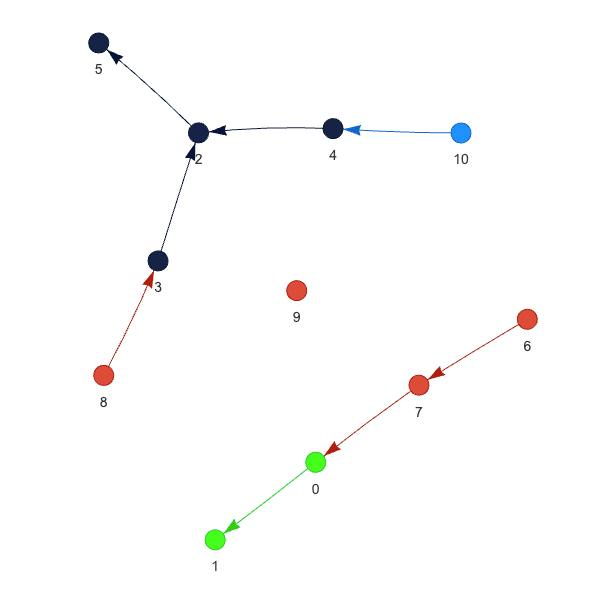
\includegraphics[width=0.3\linewidth]{fig/partial-orders.png}
    \caption{For a commit comprising of 11 edits with the dependencies specified above, there are initially 13,860 possible sequences. By applying partial-order reduction, this figure drops to only 36, reflecting a 99\% decrease in the overall search space.}
    \label{fig:partial-order}
\end{figure}

\subsection{Key Components}

\textbf{Independence}: Let \( S \) represent the set of system states and \( T \subseteq S \times S \) represent the set of transitions (or actions). Two transitions \( t_1, t_2 \in T \) are considered \textit{independent} if the following conditions hold:
\begin{enumerate}
    \item \textbf{Commutativity}: The order of execution does not affect the system's state:
    \[
    t_1(s) \xrightarrow{t_2} s' \iff t_2(s) \xrightarrow{t_1} s'
    \]
    where \( t_1(s) \) represents the state resulting from applying \( t_1 \) to state \( s \).
    \item \textbf{Non-interference}: Execution of one transition does not disable the other:
    \[
    t_1 \text{ is enabled in state } s \implies t_2 \text{ is also enabled in } t_1(s).
    \]
\end{enumerate}

\textbf{Dependency}: Two transitions \( t_1, t_2 \) are \textit{dependent} if they do not satisfy the independence conditions. Dependency implies that the order of execution can affect the system state. 

\textbf{Equivalence Classes of Executions}: Define an equivalence relation \( \sim \) over the set of executions based on their observable behavior. Two executions \( \sigma_1 \) and \( \sigma_2 \) are equivalent if they differ only in the order of independent transitions:
\[
\sigma_1 \sim \sigma_2 \iff \text{same final state and equivalent under reordering of independent transitions.}
\]

\textbf{Reduction Criterion}: For a given state \( s \), a reduced set of transitions \( T_{\text{red}}(s) \subseteq T \) is selected such that every equivalence class of executions contains at least one representative path that is explored. This ensures \textit{state space preservation}:
\[
\forall t \in T, \exists t' \in T_{\text{red}}(s): \quad t \sim t'.
\]
\subsection{Workflow}

Given a system \( (S, T, s_0) \), where \( S \) is the set of states, \( T \) is the set of transitions, and \( s_0 \) is the initial state:
\begin{enumerate}
    \item \textbf{Dependency Analysis:} Compute the dependency relation \( \mathcal{D} \subseteq T \times T \) based on independence criteria.
    \item \textbf{Ample Set Selection:} For each state \( s \), select a subset of transitions \( \text{Ample}(s) \subseteq T \) such that:
    \begin{itemize}
        \item \textit{Enabledness}: \( \text{Ample}(s) \) includes only transitions enabled in \( s \).
        \item \textit{Dependency Coverage}: If a transition $t \notin Ample(s)$ is dependent on a transition in $Ample(s)$, $t$ must be eventually explored through the reduced state space.
        \item \textit{Cycle Freedom}: The reduced state space must remain acyclic under certain conditions.
    \end{itemize}
    \item \textbf{State Exploration:} Explore only the transitions in \( \text{Ample}(s) \) for each state \( s \).
    \item \textbf{Pruning:} Avoid re-exploring states that are equivalent under the equivalence relation \( \sim \).
\end{enumerate}

\subsection{Preservation Properties}
Partial Order Reduction guarantees\footnote{The full proof of the liveness and safety properties can be found in Appendix A} the preservation of certain properties in the reduced state space:
\begin{itemize}
    \item \textbf{Safety:} If the original system satisfies a safety property (e.g., no deadlock), the reduced system will also satisfy it.
    \item \textbf{Liveness:} If the original system satisfies liveness properties (e.g., progress), the reduced system will as well.
\end{itemize}

Formally:
\[
\forall \phi \in \mathcal{P}: \quad (S, T, s_0) \models \phi \iff (S_{\text{red}}, T_{\text{red}}, s_0) \models \phi
\]
where \( \mathcal{P} \) is the set of properties being verified.

\subsection{Directed Acyclic Graph}
The dependency relationships derived through POR can be represented as a Directed Acyclic Graph: 
\begin{itemize}
    \item \textbf{Nodes}: Represent individual edits $h_i \in \mathbf{H}$
    \item \textbf{Edges}: Represent transitions $h_i \rightarrow h_j$, indicating that $h_i$ must occur before $h_j$
\end{itemize}

\section{Dependency Analysis}
We present the observations and work to formalize the various types of dependencies.

\subsection{Observations}

The following are key observations (examples provided in Figure \ref{fig:observations}):

\begin{enumerate}
    \item A single edit region may contain multiple edit semantics, which may require multiple rounds of parsing before full processing.
    \item The order of edits should be arranged based on their dependencies to ensure correct sequencing.
    \item Independent edits can be applied concurrently with no regards to consequences.
    \item Edits within the same code block are more likely to occur sequentially due to their local dependencies and proximity.
    \item Inter-file dependencies are often mediated through shared components (e.g., imports, global variables, or shared libraries).
\end{enumerate}


\begin{figure}%
    \centering
    \subfloat[\centering One edit region may contain multiple edit semantic, that may be visited twice]{{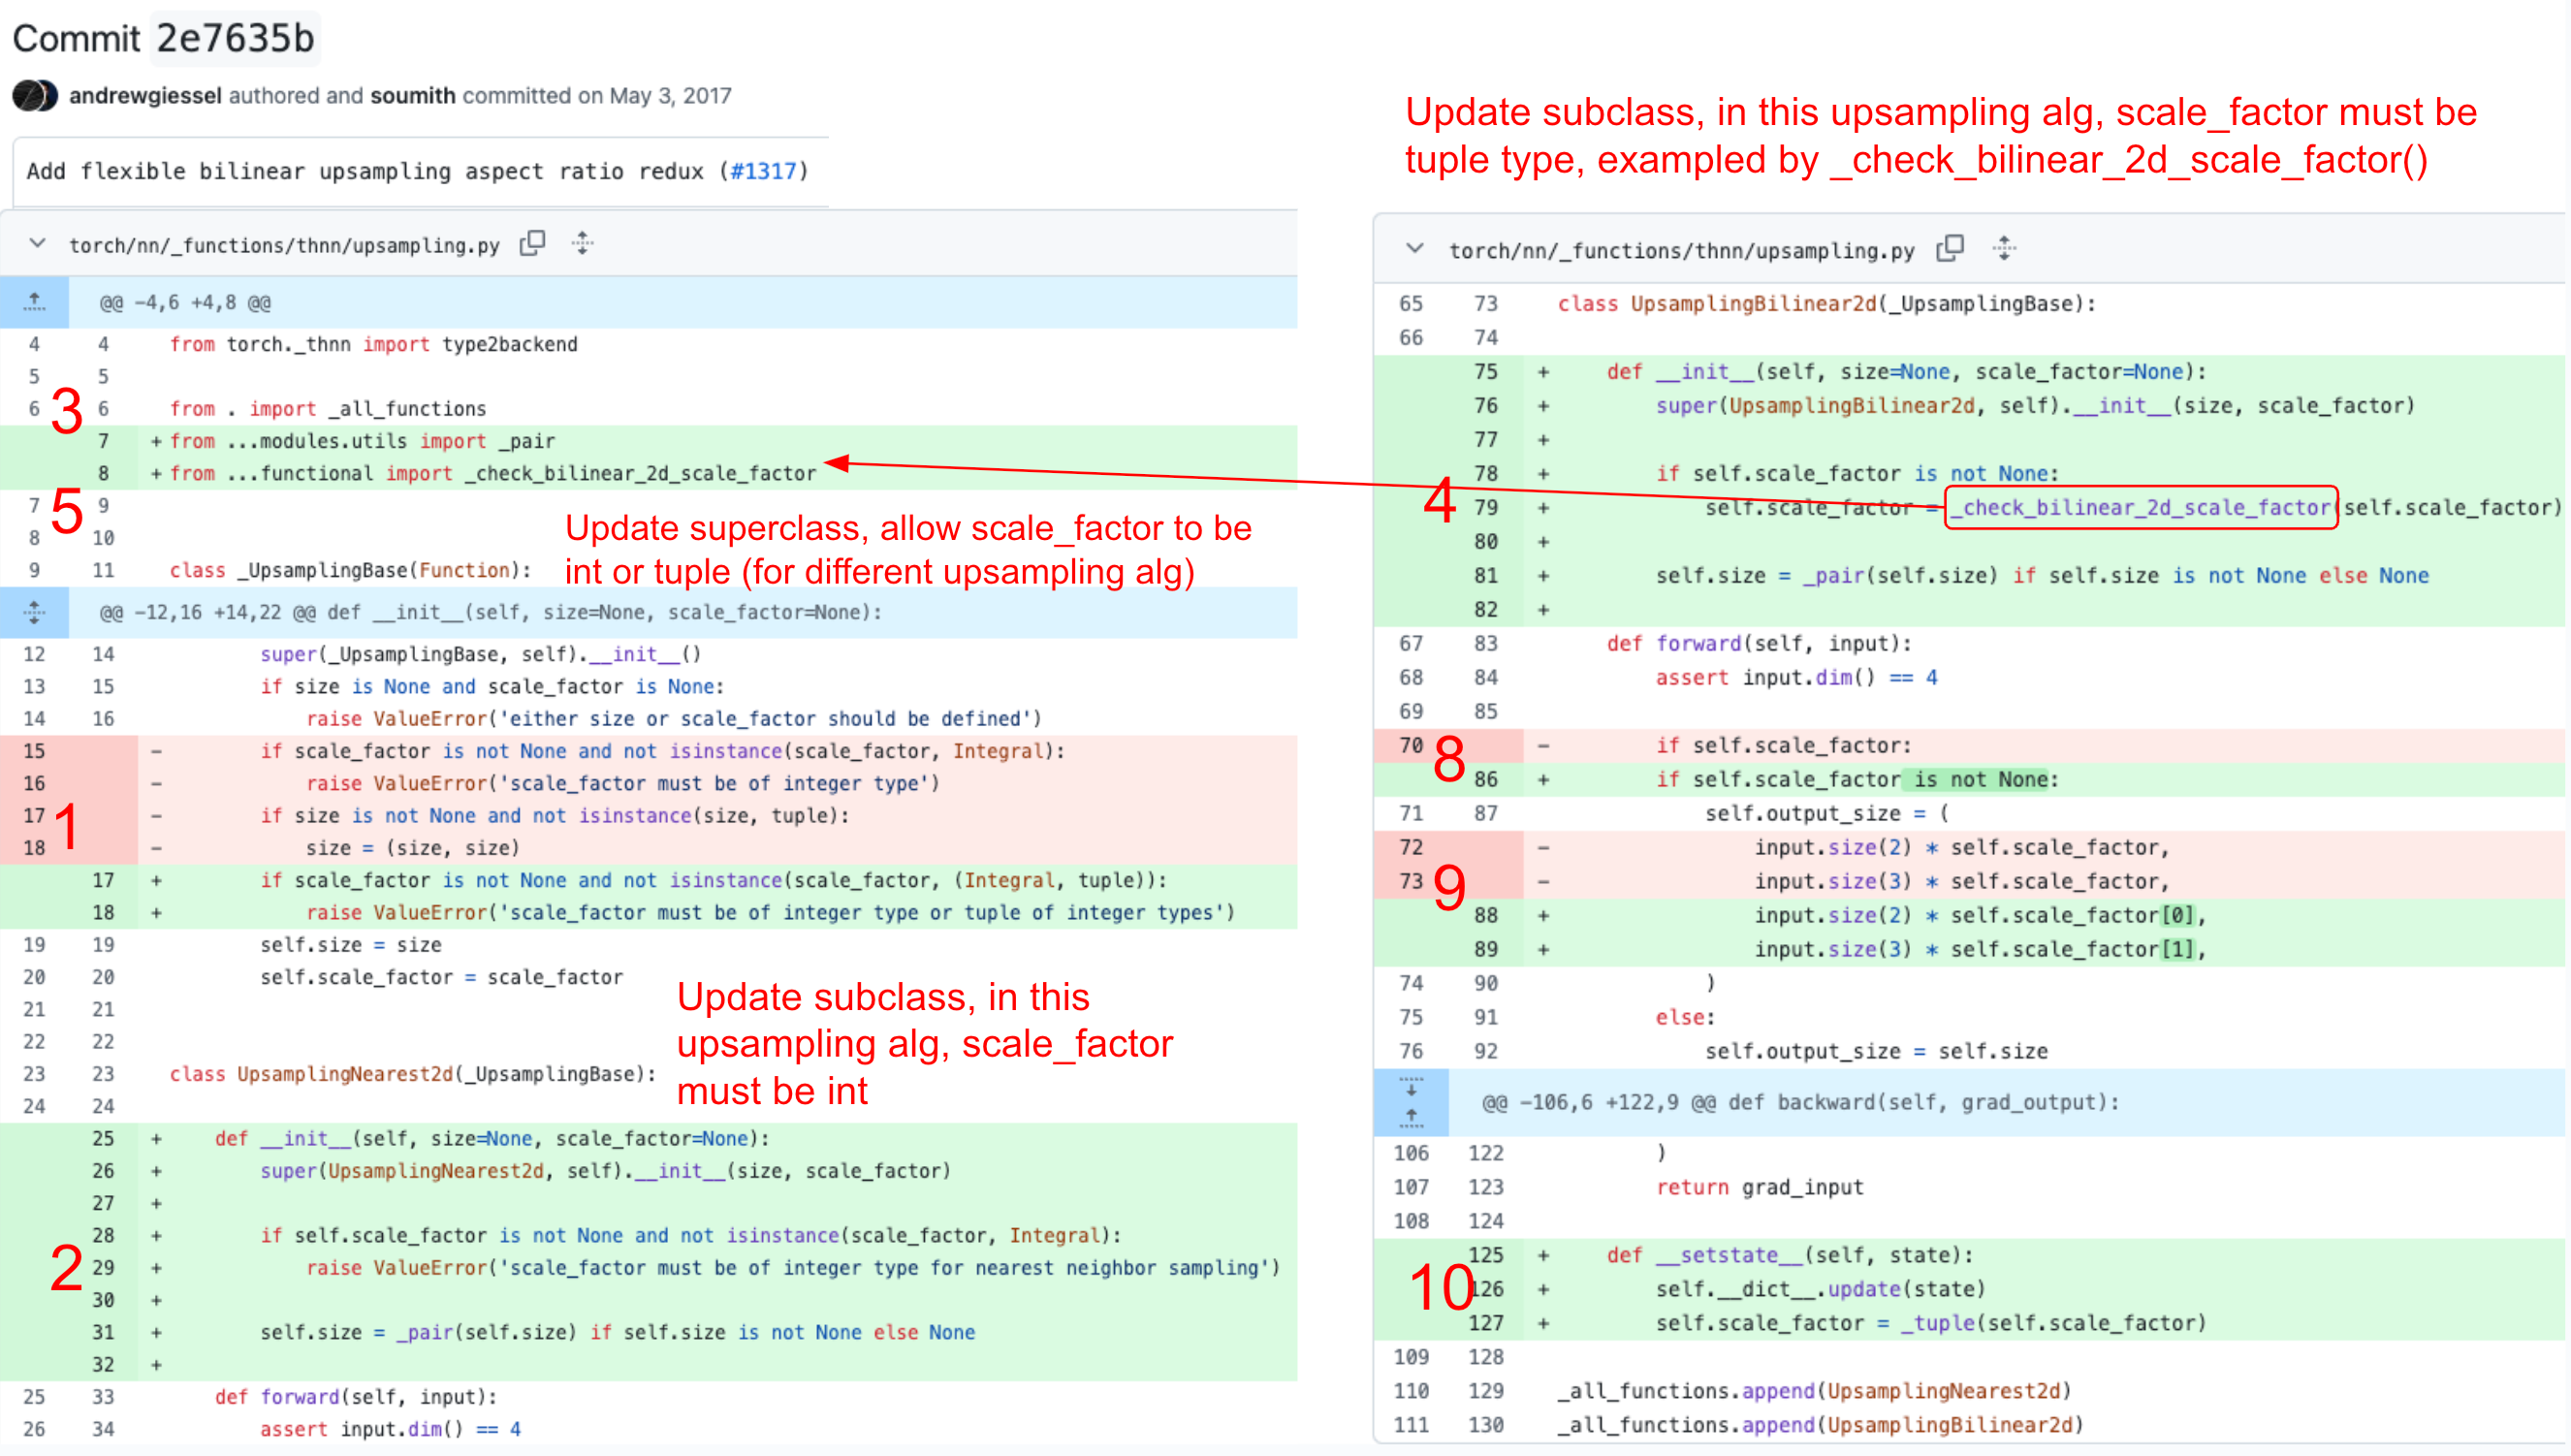
\includegraphics[width=9cm]{fig/obs_1.1.png} }}%
    \qquad
    \subfloat[\centering Arrange edit order by their dependency]{{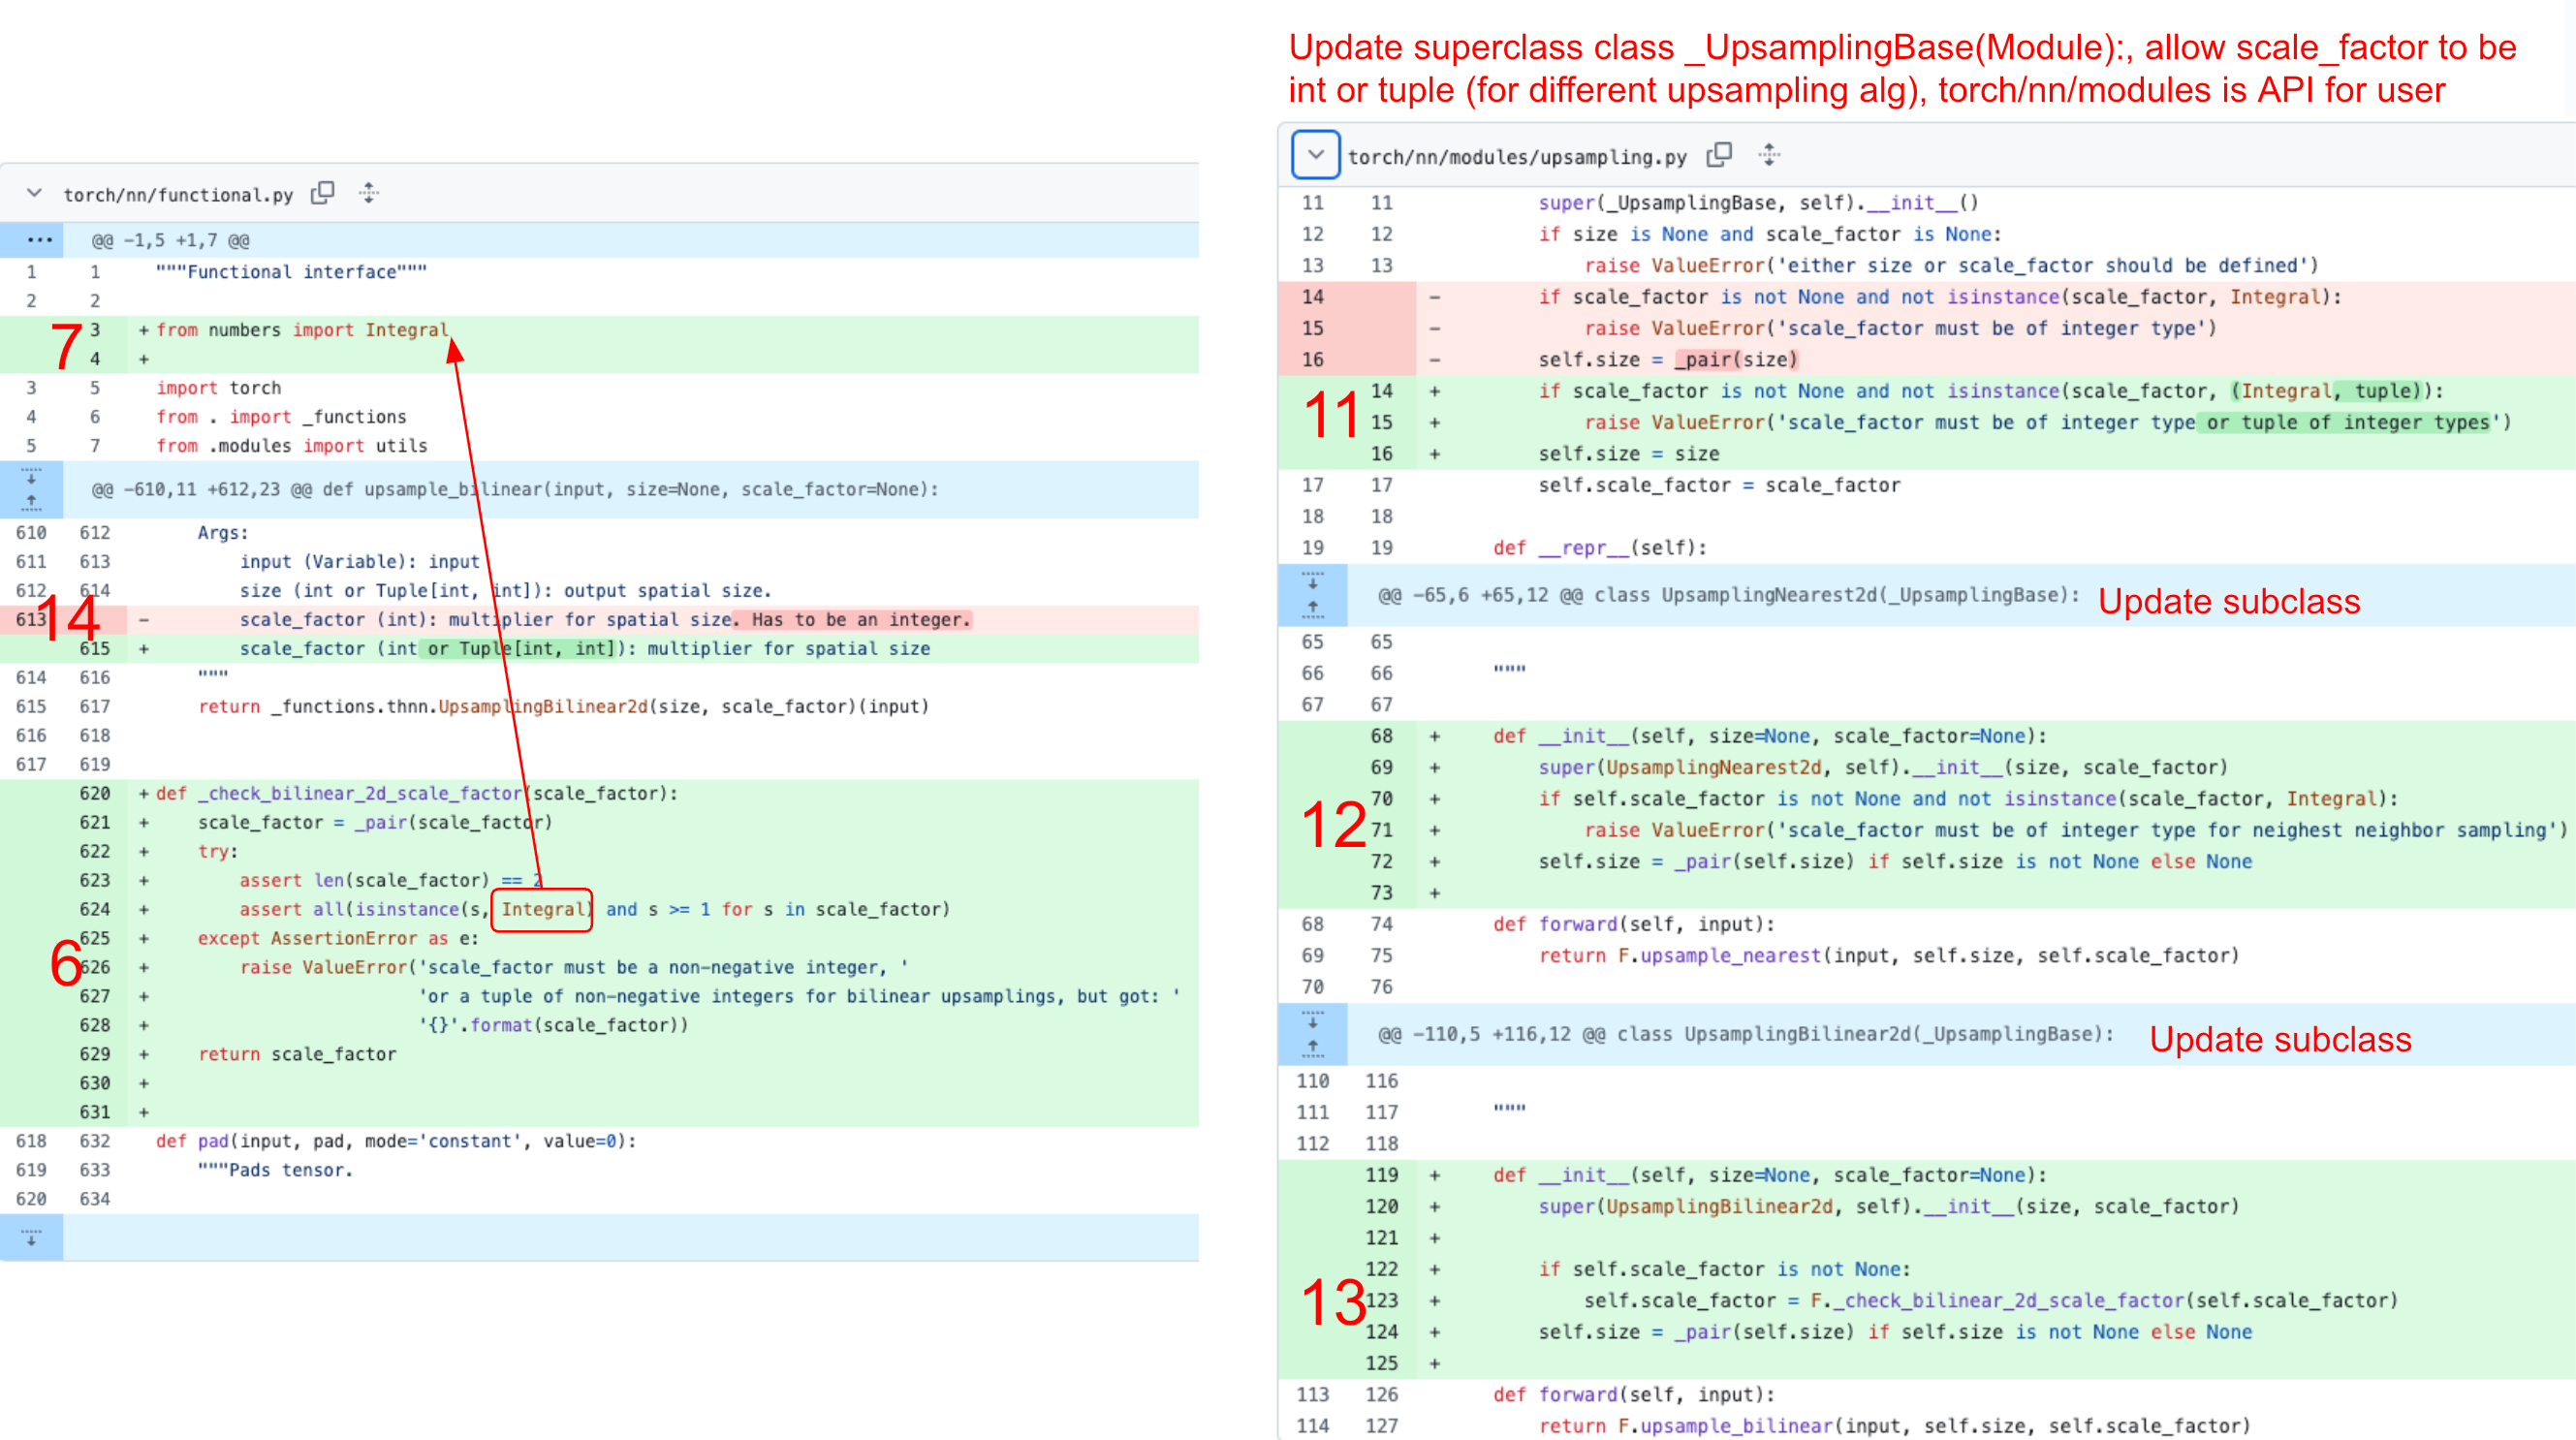
\includegraphics[width=9cm]{fig/obs_1.2.png} }}%
    \qquad
    \subfloat[\centering Parallelism between similar edit compositions]{{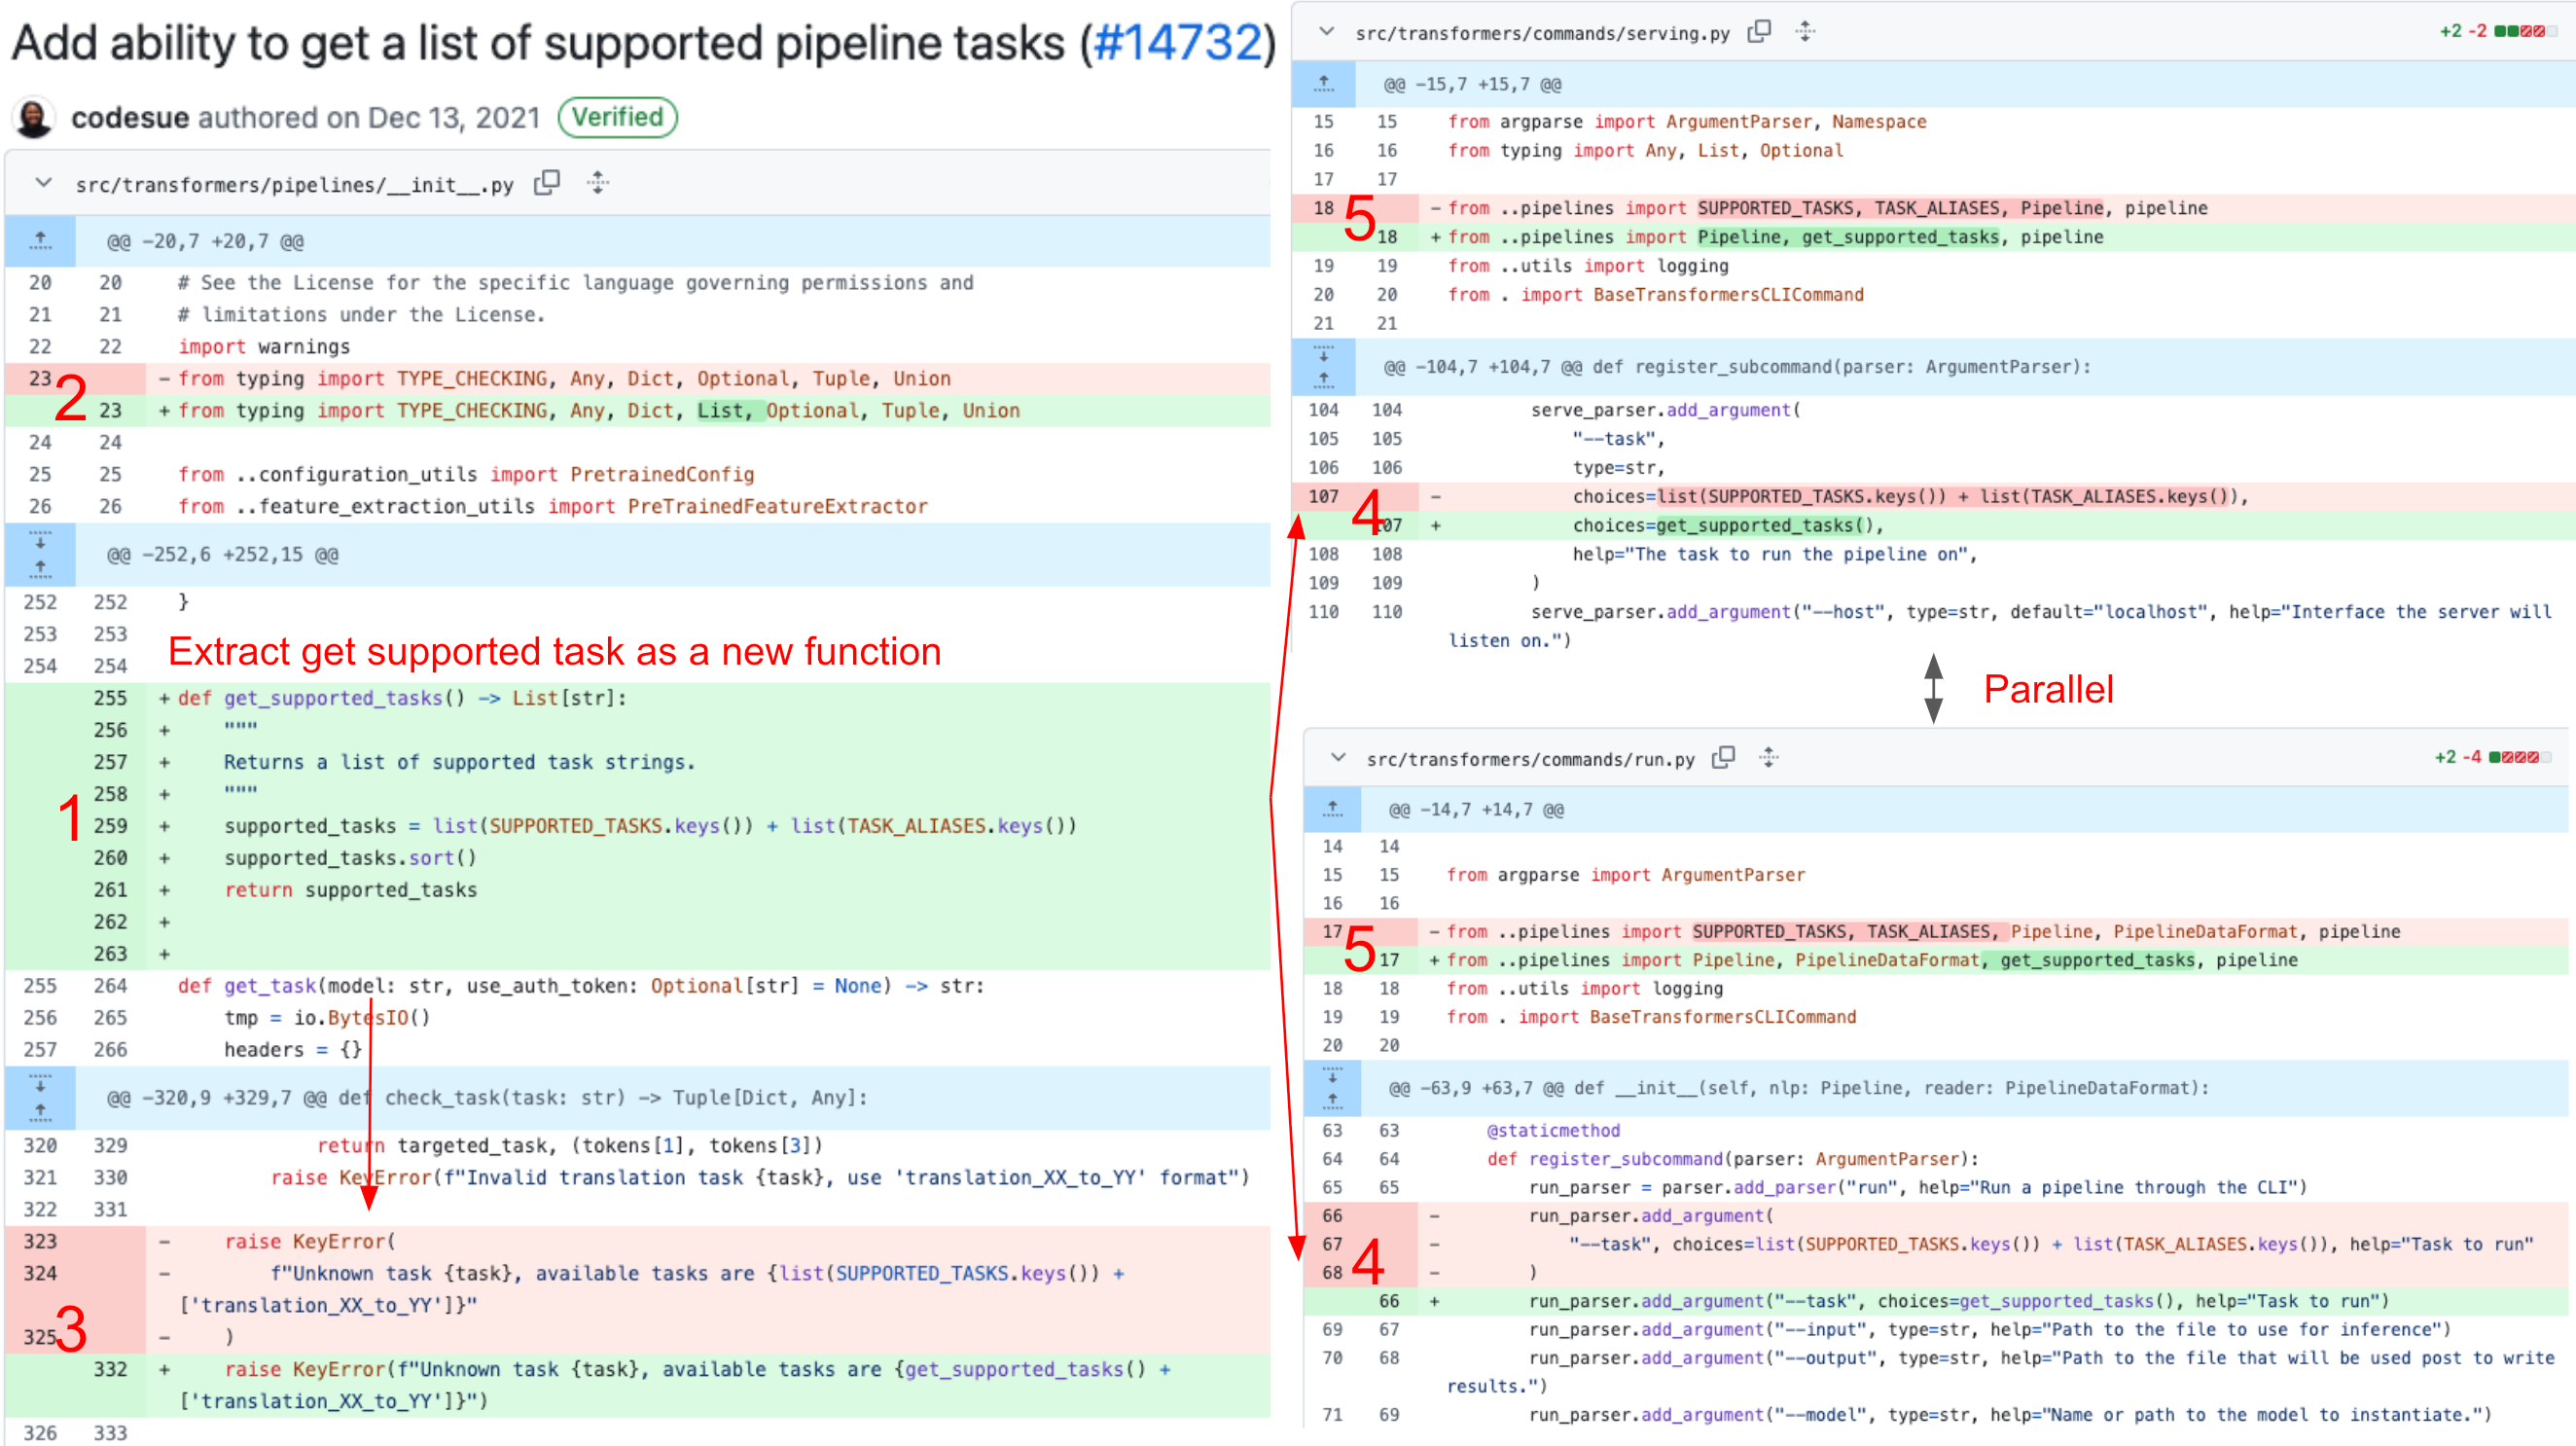
\includegraphics[width=9cm]{fig/obs_1.3.png} }}%
    \qquad
    \subfloat[\centering Edits in the same block are more likely to happen in sequential order]{{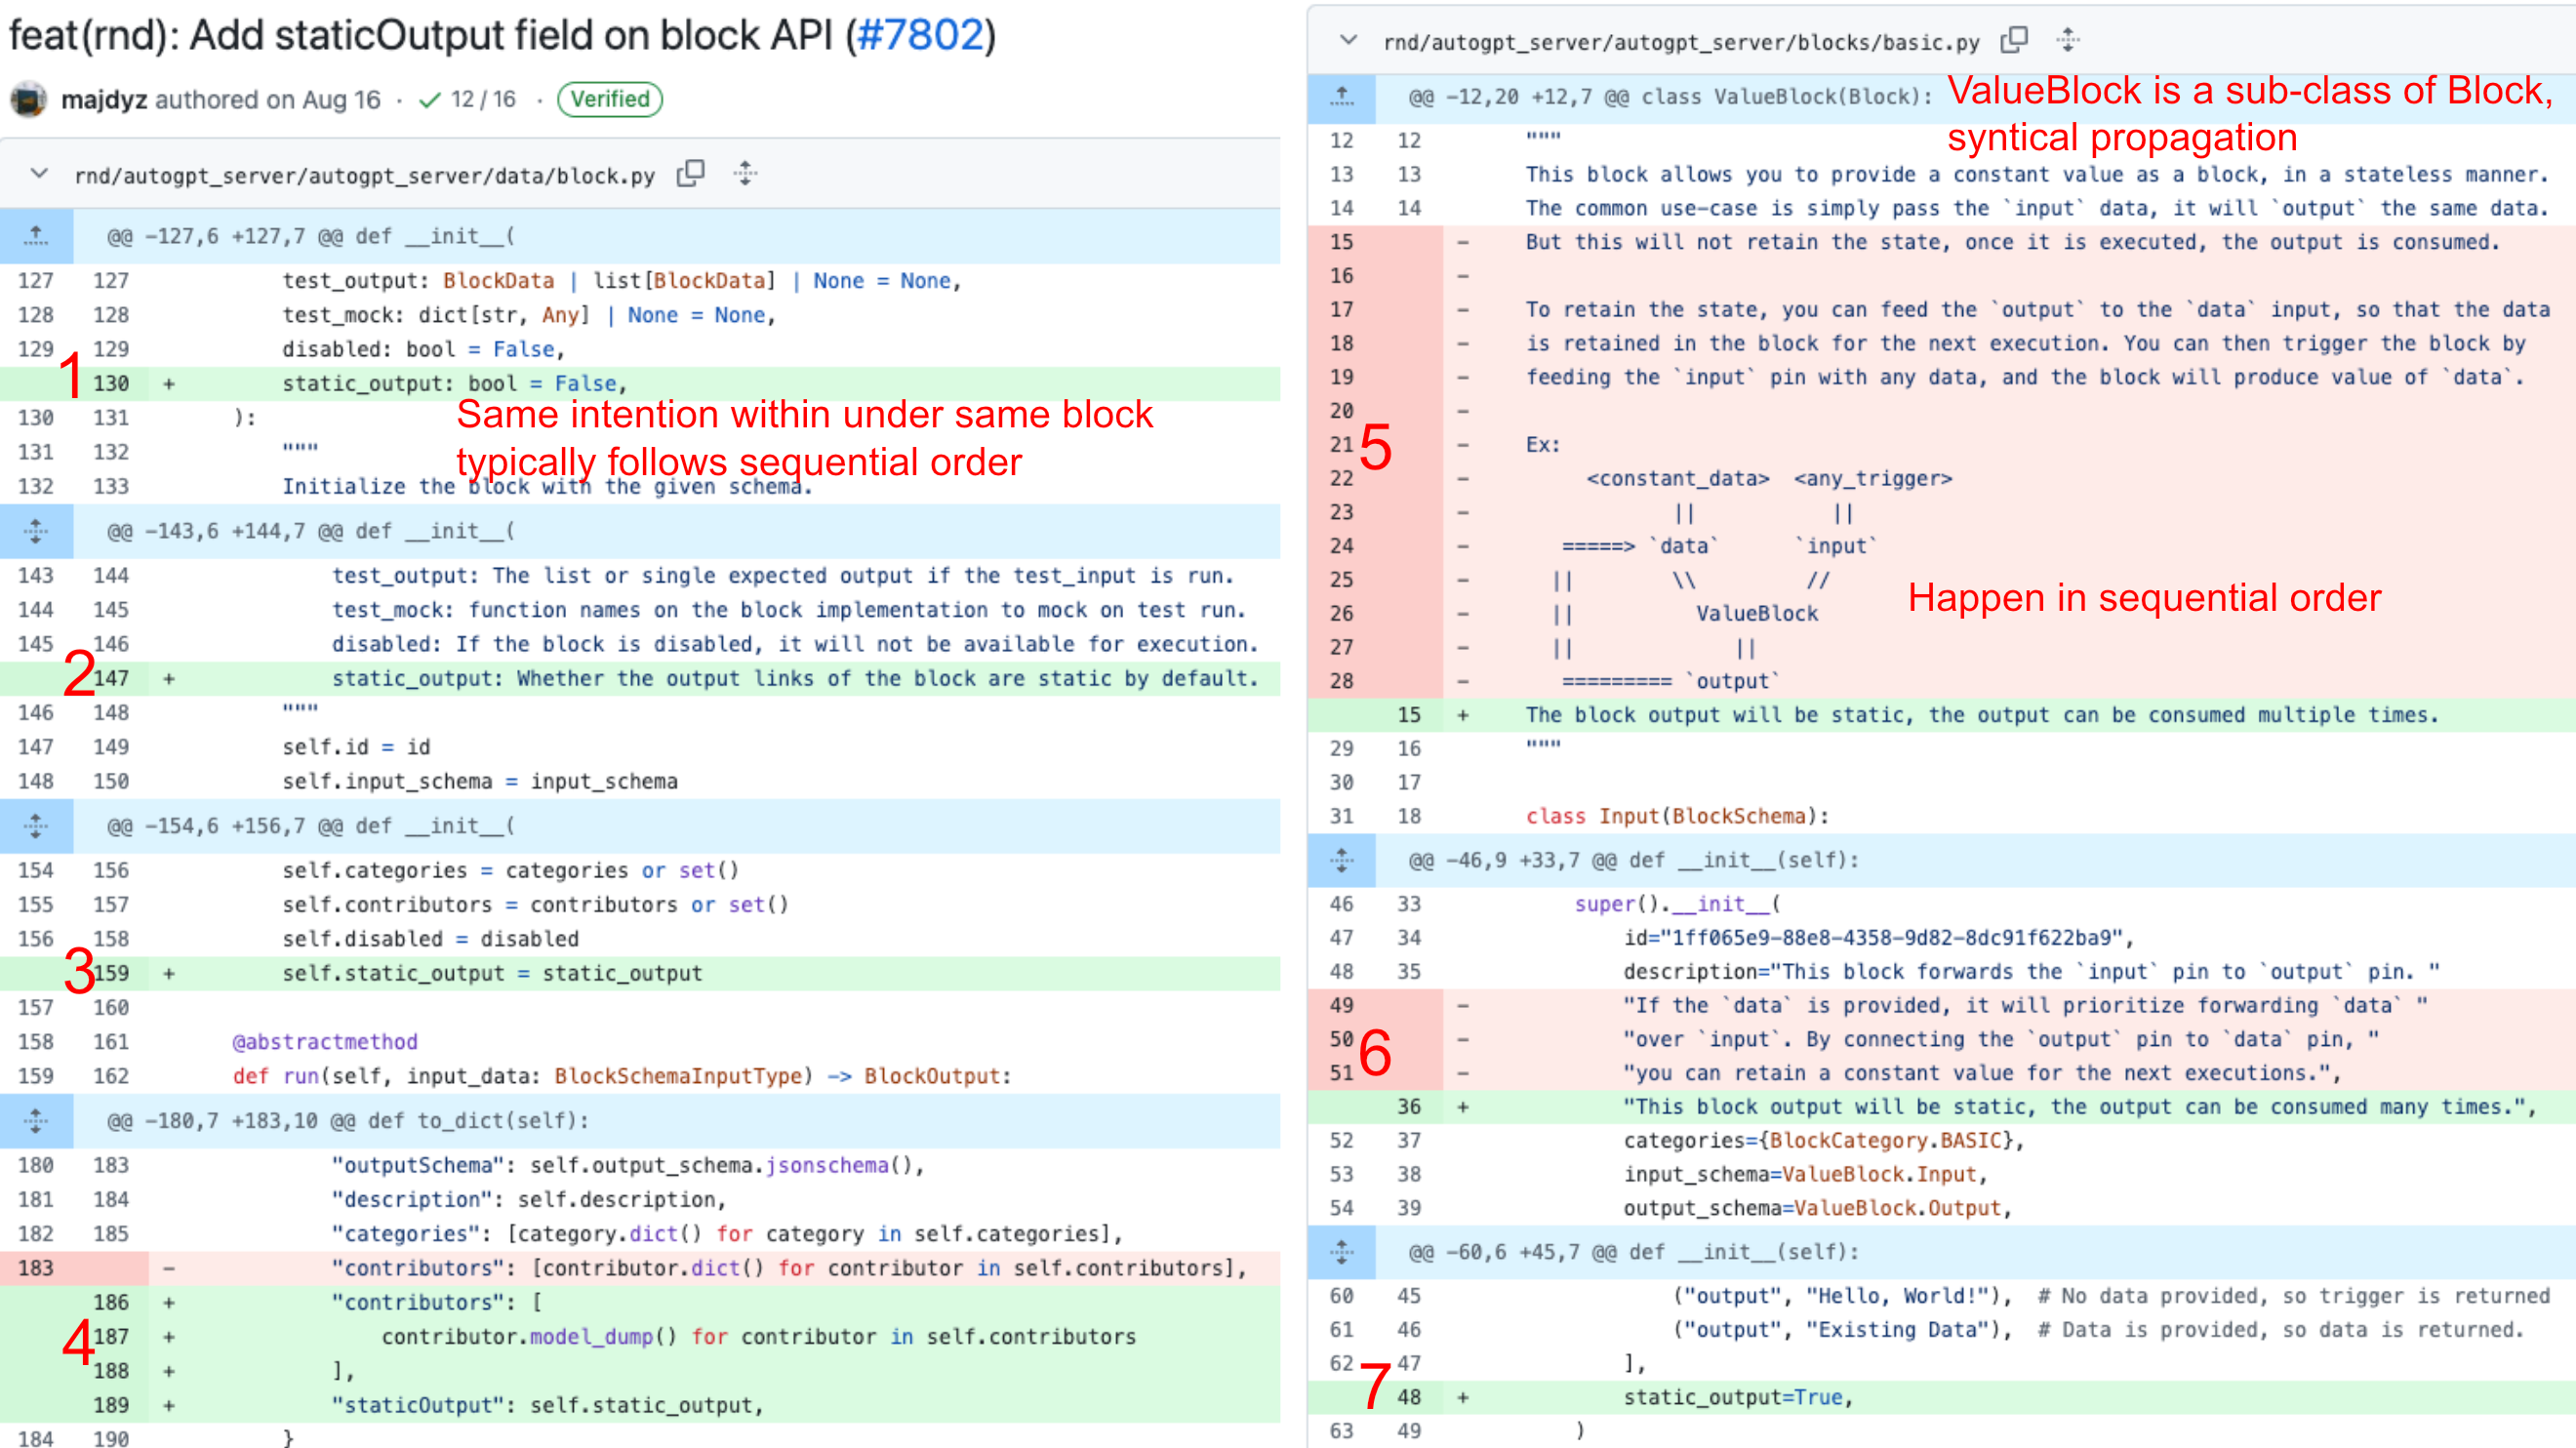
\includegraphics[width=9cm]{fig/obs_1.4.png} }}%
    \caption{Observations}%
    \label{fig:observations}%
\end{figure}


% \begin{figure}
%     \centering
%     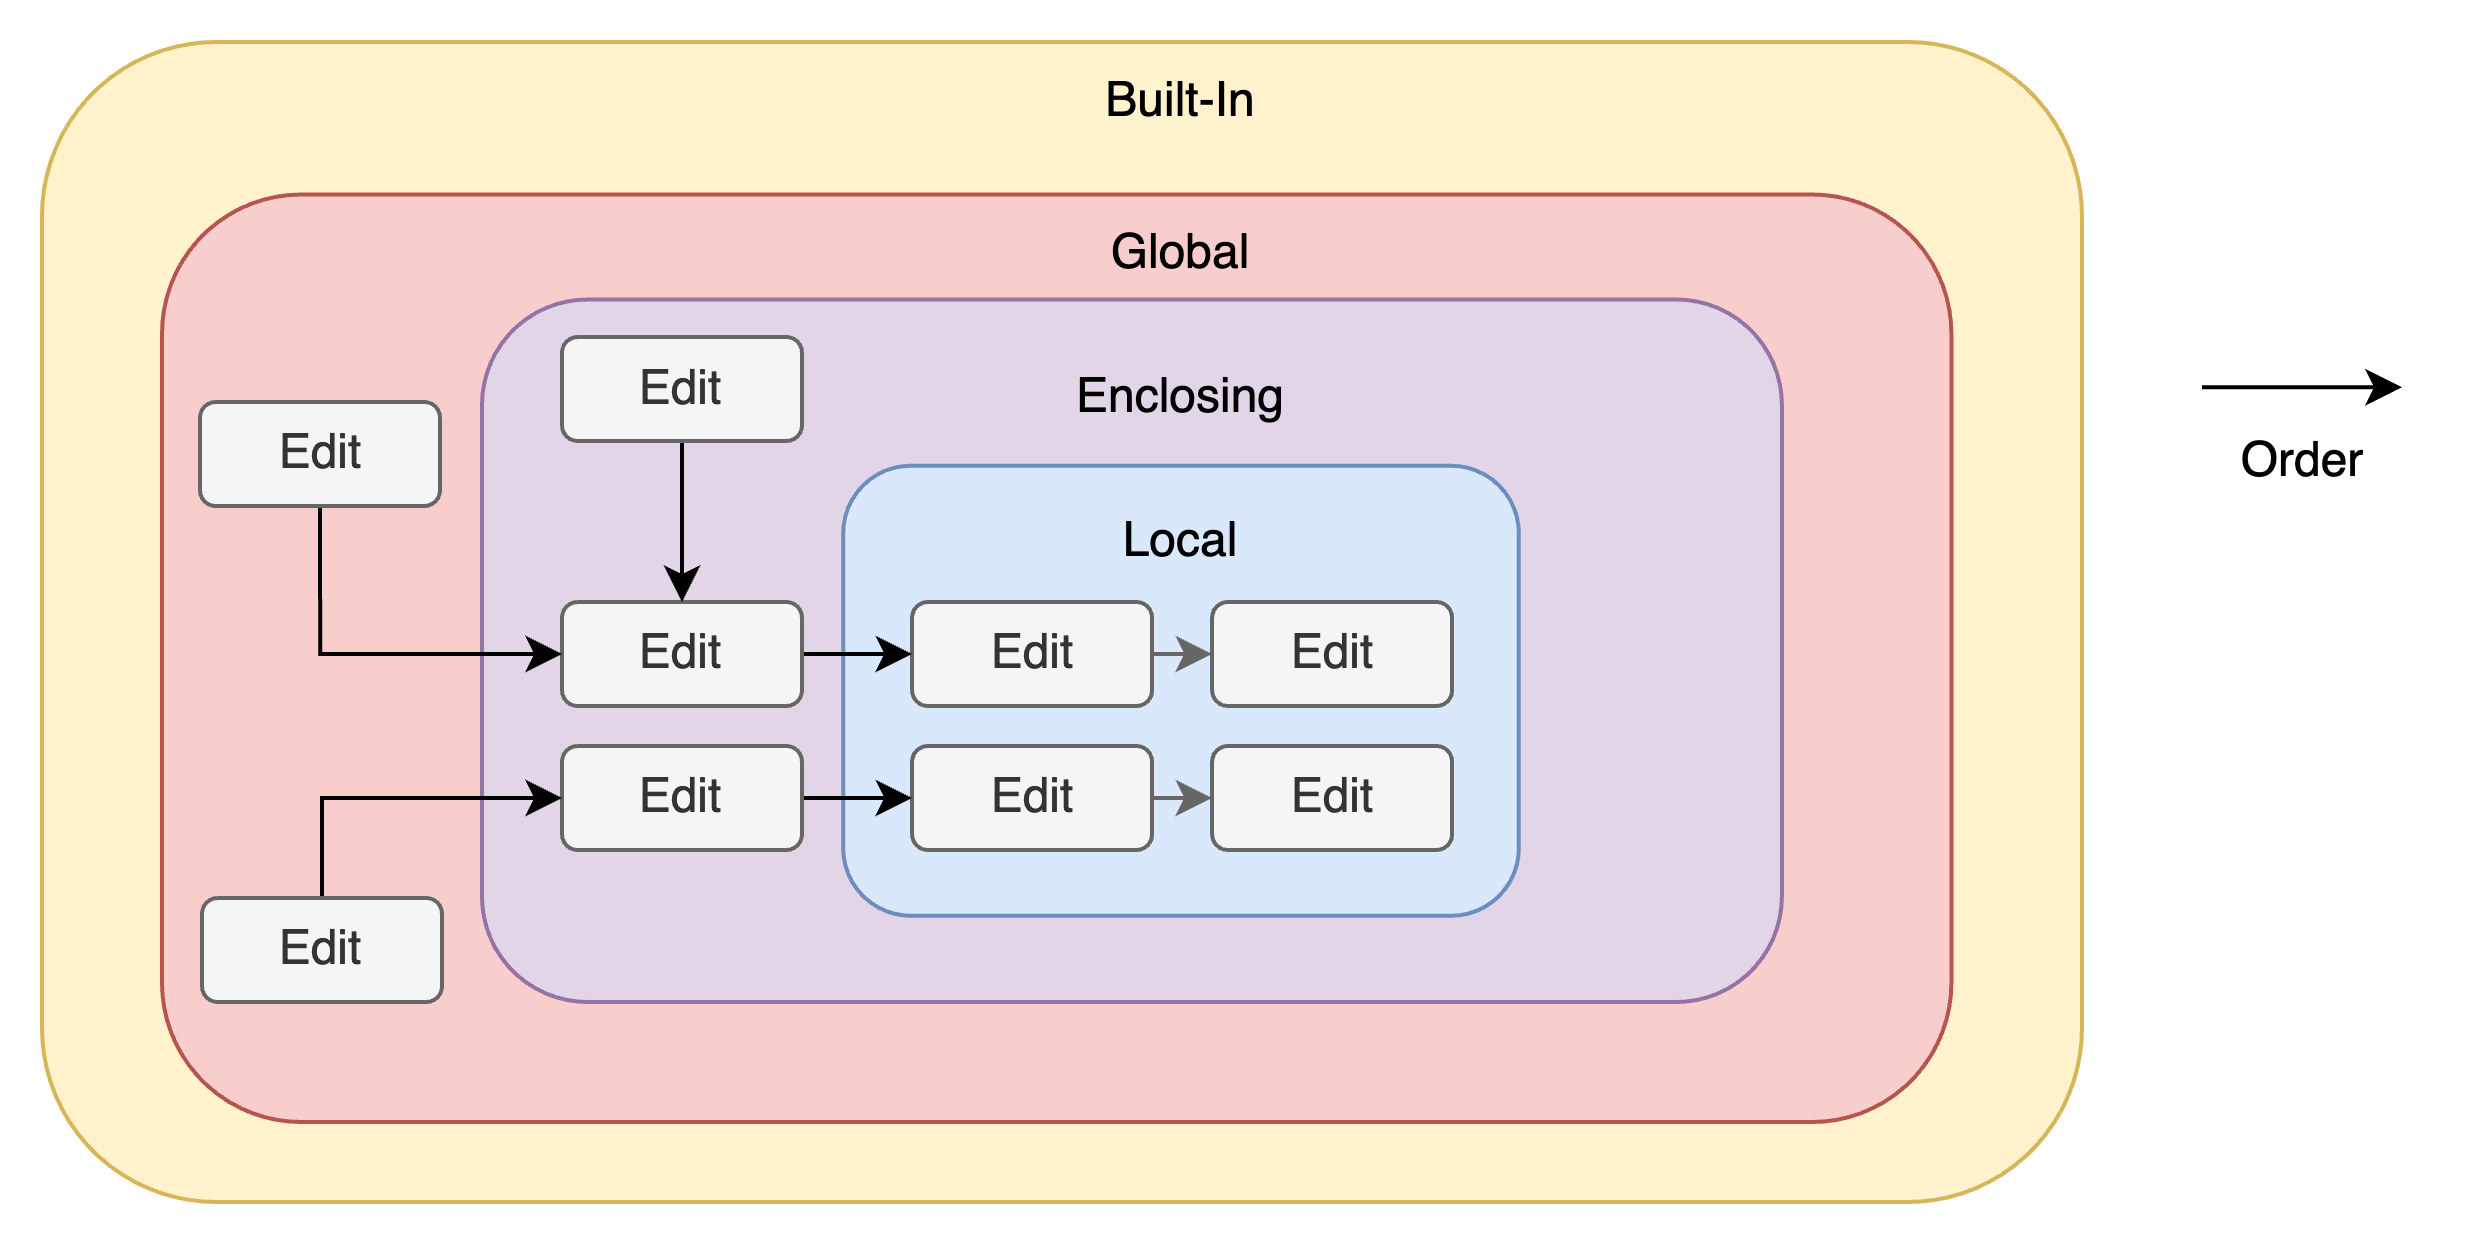
\includegraphics[width=0.6\linewidth]{fig/code_proximity.png}
%     \caption{Code proximity and dependencies}
%     \label{fig:proximity}
% \end{figure}

\subsection{Types of Dependencies}

Given the above observations, we further categorized these edits into three types of dependencies: Syntactic, Semantic, and Proximity. Given two elements \( h_i, h_j \in \mathbf{H} \), the type of relationship between them is defined by a function \( f(h_i, h_j) \) as follows:

\subsubsection{Syntactic Dependency}
Syntactic dependencies arise from structural relationships within the abstract syntax tree (AST). These include:
\begin{itemize}
    \item \textbf{Variable:} Relationships between variable declarations and their usages.
    \item \textbf{Control Flow:} Dependencies introduced by constructs such as loops or conditional statements.
    \item \textbf{Scope:} Relationships governed by scope hierarchies, such as nested blocks or functions.
\end{itemize}
For example, an edit modifying a loop header might syntactically depend on edits to its body.

\subsubsection{Semantic Dependency}
Semantic dependencies are derived from the meaning and behavior of the code. These include:
\begin{itemize}
    \item \textbf{Type:} Relying on type definitions or changes (e.g., updating function signature affects call sites).
    \item \textbf{Execution Flow:} Relationships influenced by control flow or data flow analysis.
    \item \textbf{Functional Relationships:} Dependencies between a function definition and its invocations.
\end{itemize}
For example, if \( h_i \) modifies a function’s logic and \( h_j \) updates a related test case, they are semantically dependent.

\subsubsection{Proximity Dependency}
Proximity dependencies are based on the physical closeness of edits in the codebase. These dependencies often arise due to:
\begin{itemize}
    \item \textbf{Local Context:} Edits within the same function, class, or block of code.
    \item \textbf{Spatial Relationships:} Edits located near each other in terms of line numbers or columns.
\end{itemize}
For example, two edits \( h_i \) and \( h_j \) that update consecutive lines in the same block likely exhibit a proximity dependency.

\subsubsection{No Dependency}
If \( f(h_i, h_j) = \emptyset \), there is no direct relationship between the edits \( h_i \) and \( h_j \). These edits can be applied independently without affecting the correctness of the codebase.

\subsection{Dependency Matrix Representation}
To facilitate the analysis and visualization of dependencies, we construct a dependency matrix \( D \), where each element \( D_{ij} \) represents the dependency type between \( h_i \) and \( h_j \):
\[
D_{ij} =
\begin{cases}
    \text{1}, & \text{if } f(h_i, h_j) \neq \emptyset \\
    \text{0}, & \text{if } f(h_i, h_j) = \emptyset
\end{cases}
\]
Additionally, the dependency type can be encoded in \( D \) as categorical values, where:
\[
D_{ij} =
\begin{cases}
    \text{S}, & \text{if Syntactic Dependency exists} \\
    \text{M}, & \text{if Semantic Dependency exists} \\
    \text{P}, & \text{if Proximity Dependency exists} \\
    \emptyset, & \text{if no dependency exists.}
\end{cases}
\]
This matrix provides a compact representation of the relationships between edits and serves as input for further analysis or optimization algorithms.


% \subsubsection{Syntactic Dependency}
% A modification in one code segment propagates to other areas that depend on it. If a code segment \( h_i \) is altered and another segment \( h_j \) depends on it, then \( h_j \) may experience compilation or runtime errors if the dependency is not addressed. This type of propagation is directional:
%    \[
%    h_i \rightarrow_{\text{dep}} h_j \text{ if } h_j \text{ has a dependency on } h_i.
%    \]
% \subsubsection{Logical Dependency}
% In cases where a modification in one code segment \( h_i \) requires additional implementation in other segments to fulfill the intended functionality, we define this as logical propagation. This type does not lead to immediate errors but results in incomplete functionality until all related edits are made. Here, \( h_i \) logically precedes \( h_j \):
%    \[
%    h_i \rightarrow_{\text{log}} h_j \text{ if } h_j \text{ logically completes the function of } h_i.
%    \]

% \subsubsection{Semantic Dependency} 

% A modification in one code segment \( h_i \) may influence other segments \( h_j \) with similar code patterns, even if they are not directly related by dependency or logic. These edits share similar semantics, and the propagation is generally applied bidirectionally:
%    \[
%    h_i \leftrightarrow_{\text{sem}} h_j \text{ if } h_i \text{ and } h_j \text{ share semantic similarity and influence each other bi-directionally.}
%    \]


\section{Dependency Derivation}

In this section, different methods were explored and their results were aggregated to estimate the dependency between two different edits, $h_i, h_j \in \mathbf{H}$. 


\subsection{Heuristics}

The heuristic approach leverages observed patterns to establish a relative ordering of edits, denoted as \(\mathbf{H} = \{ h_1, h_2, \dots, h_n \}\). For each edit \( h_i \in \mathbf{H} \), we categorize the edit type (addition, deletion, or modification) and prioritize the ordering based on the following observations:

\begin{enumerate}
\item \textbf{Edit Priority}: Deletions \( h_i \in \mathbf{H}_{\text{del}} \) precede additions \( h_i \in \mathbf{H}_{\text{add}} \). Thus, for any two edits \( h_i, h_j \in \mathbf{H} \), if \( h_i \in \mathbf{H}_{\text{del}} \) and \( h_j \in \mathbf{H}_{\text{add}} \), we have \( h_i \rightarrow h_j \).
\item \textbf{Top-Down Order}: Edits within a single file are applied from top to bottom, yielding an order based on line numbers \( \text{line}(h_i) < \text{line}(h_j) \implies h_i \rightarrow h_j \).
\item \textbf{Import Order}: If \( h_i \) involves a module import and \( h_j \) references it, we establish \( h_i \rightarrow h_j \) based on the dependency.
\item \textbf{Lint Errors:} Procedurally sample across a set of error-free edits \( E = \{e_1, e_2, \dots, e_n\} \) to iteratively construct a valid program \( P = \{p_1, p_2, \dots, p_m\} \), where each intermediate program \( p_j \) is error-free \cite{jimenez2023, pandey2024}.
\item \textbf{Identical Code}: Let $\mathcal{E} = \{e_1, e_2, \dots, e_n\}$ be the set of edits and define $\mathrm{Code}(e_i)$ as the code produced by edit $e_i$. We say that two edits are redundant if 
\[
e_i \sim e_j \quad \Longleftrightarrow \quad \mathrm{Code}(e_i) \equiv \mathrm{Code}(e_j),
\]
where $\equiv$ denotes identical or semantically equivalent code. Merge each equivalence class $[e] = \{e_i \in \mathcal{E} \mid e_i \sim e\}$ into a single representative edit to minimize redundancy and reduce conflicts.
\end{enumerate}


The resultant ordering, \( O_{\text{heuristic}}(\mathbf{H}) \), provides a sequence based on these heuristic rules. 

\subsection{Static Analysis}

The static analysis approach utilizes the set of heuristics identified in the previous section to explicitly identify \textit{possible} dependencies between edits. We define a parser \( P(h_i, h_j) \) to estimate the dependency between two edits \( h_i \) and \( h_j \) by performing the following steps:

\begin{enumerate}
    \item \textbf{Abstract Syntax Tree (AST) Generation:}  
    The parser \( P \) first generates an abstract syntax tree (AST)\footnote{An abstract syntax tree is a tree representation of the syntactic structure of source code, commonly used in compilers and static analysis tools.} (Figure \ref{fig:dependency_graph}) for the source code, capturing structural relationships such as nested blocks, function definitions, and variable declarations.

    \item \textbf{Edit Position and Identifier Extraction:}  
    Using the AST, \( P \) identifies the positions (e.g., line and column numbers) and constructs identifiers\footnote{Identifiers are unique names assigned to variables, functions, or other entities in the code to facilitate tracking and analysis.} for each edit \( h_i \). This information establishes a mapping between the edits and their respective code regions.

    \item \textbf{Dependency Tracing with Language Server Protocol (LSP):}  
    Leveraging the Language Server Protocol (LSP)\footnote{LSP is a protocol standard for language-agnostic static analysis and editor integrations, enabling features like auto-completion, go-to-definition, and dependency tracing.}, the parser traces dependencies by analyzing cross-references, type hierarchies, and function calls between \( h_i \) and \( h_j \). This step captures both local (intra-file) and global (inter-file) dependencies.
\end{enumerate}

\begin{figure}
    \centering
    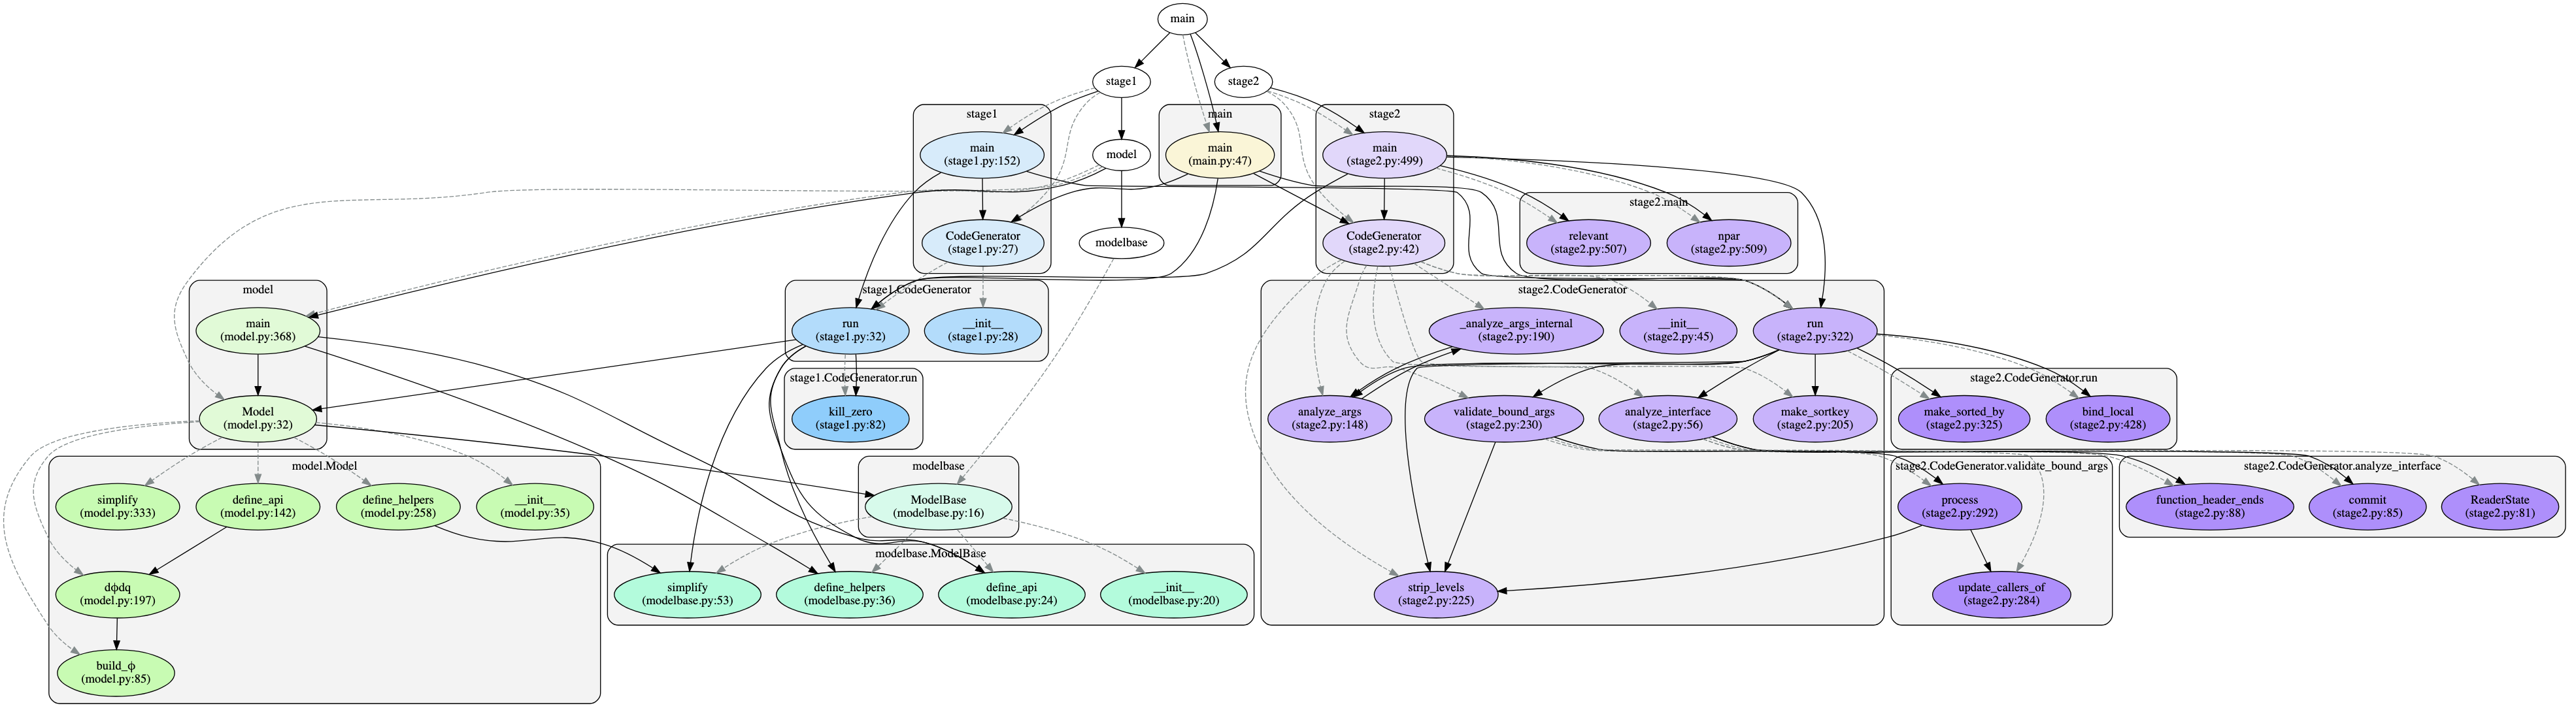
\includegraphics[width=0.8\linewidth]{fig/dependency_graph.png}
    \caption{Pyan constructs a directed graph of the objects in the combined source, and how they define or use each other}
    \label{fig:dependency_graph}
\end{figure}

\subsection{Agents}

The agentic approach uses a language model\footnote{In our experiments, we have mainly adopted GPT4, Gemini-Flash, DeepSeek v3 and Llama.} \( \mathcal{M} \) to infer relationships between edits by providing relevant context for each edit \( h_i \in \mathbf{H} \). For each edit, we create a context vector \( \mathbf{c}(h_i) \), which includes pre-existing code usage data such as function signatures or variable assignments:
\[
\mathbf{c}(h_i) = \{ \text{usage}(h_i), \text{dependencies}(h_i) \}
\]

Given the context vectors \( \mathbf{C} = \{\mathbf{c}(h_1), \mathbf{c}(h_2), \dots, \mathbf{c}(h_n)\} \), the language model \( \mathcal{M} \) attempts to establish a total order:
\[
O_{\text{agentic}}(\mathbf{H}) = \mathcal{M}(\mathbf{C})
\]

This order \( O_{\text{agentic}}(\mathbf{H}) \) reflects the language model's inferred relationships. We will be adapting the Chain of Agents (CoA) framework for multi-agent orchestration.

\section{Context Selection and Prompt Construction}

With limited context\footnote{Although Google's Gemini-Pro has a context window of 2 million token length, we have opted not to use it due to latency and limited hardware.} available, it is not feasible to utilize the entirety of a code repository or external database as input context. To address this limitation, we employ a systematic process to construct the final prompt by selecting the most relevant examples from an external vector database and the repository. This process can be formalized as follows:

\subsubsection{Input Space}
Let \( R \) represent the code repository, consisting of files \( F = \{f_1, f_2, \ldots, f_n\} \), where each file \( f_i \) contains code snippets \( S_i = \{s_{i1}, s_{i2}, \ldots\} \) and comments \( C_i = \{c_{i1}, c_{i2}, \ldots\} \). Additionally, let \( V \) denote the external vector database, consisting of collected examples \( E = \{e_1, e_2, \ldots, e_m\} \), where each example \( e_j \) is a vectorized representation of code snippets or descriptions.

\subsubsection{Relevance Selection Algorithm}
Define a relevance function \( \text{rel}(x, q) \), where \( x \) is a snippet, comment, or vectorized example, and \( q \) is the developer's query or the currently edited code context. The function evaluates the relevance of \( x \) to \( q \). Relevant snippets are selected such that:
\[
S_{\text{rel}} = \{s \in S \mid \text{rel}(s, q) > \tau_s\}, \quad C_{\text{rel}} = \{c \in C \mid \text{rel}(c, q) > \tau_c\}, \quad E_{\text{rel}} = \{e \in E \mid \text{rel}(e, q) > \tau_e\},
\]
where \( \tau_s \), \( \tau_c \), and \( \tau_e \) are predefined thresholds for relevance.

\subsubsection{Ranking}
A ranking function \( \text{rank}(x) \) assigns a priority score\footnote{We experimented with different ranking functions, particularly MSE, MAE etc.} to each selected snippet \( s \in S_{\text{rel}} \), comment \( c \in C_{\text{rel}} \), and example \( e \in E_{\text{rel}} \). The elements are sorted in descending order of their relevance:
\[
\text{rank}(S_{\text{rel}} \cup C_{\text{rel}} \cup E_{\text{rel}}) = \text{sort}\big(S_{\text{rel}} \cup C_{\text{rel}} \cup E_{\text{rel}}, \text{by } \text{rank}(x)\big).
\]

\subsubsection{Filtering}
To ensure the final prompt fits within the context window \( W_{\text{max}} \), a filtering function \( \text{filter}(X, W_{\text{max}}) \) selects the highest-ranked elements from \( X = S_{\text{rel}} \cup C_{\text{rel}} \cup E_{\text{rel}} \) such that:
\[
\sum_{x \in X'} \text{len}(x) \leq W_{\text{max}},
\]
where \( \text{len}(x) \) denotes the token length of \( x \), and \( X' \subseteq X \) is the filtered subset.

\subsubsection{Prompt Assembly}
The final prompt \( P \) is constructed by concatenating the filtered snippets, comments, and examples in their ranked order:
\[
P = \text{concat}(X').
\]

This approach ensures that the final prompt includes the most relevant information from both the repository and the external vector database. The final prompt can be found in Appendix B.